\section{Simulazioni modello di Ising 2D}

Prima di iniziare lo studio computazionale del modello, è stata eseguita la necessaria determinazione dei 
parametri simulativi ottimali. In questa fase ho considerato, sia per l'algoritmo di Metropolis che per quello 
di Wolff, reticoli $N \times N$ con 

$$
N \in \left\{100,\,200,\,300,\,400,\,500\right\}
$$

alle temperature

$$
T \in \left\{1.0,\,1.5,\,2.0,\,2.5,\,3.0,\,3.5\right\}
$$

I risultati ottenuti in questa fase sono riportati in modo rissuntivo nelle seguenti figure, delle quali la 
prima è relativa al metodo di Metropolis, mentre la seconda a quello di Wolff.

\begin{figure}[H]
    \centering
    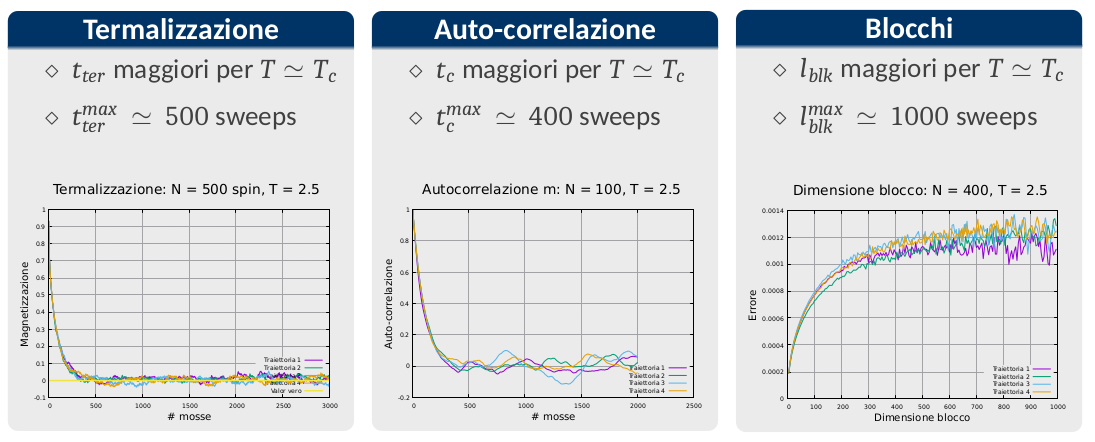
\includegraphics[width=\textwidth]{Immagini/simIsing2D/carMetro.png}
    \caption{Caratterizzazione metodo di Metropolis}
    \label{fig: magn_Ising2D}
\end{figure}



\subsection{Osservabili}

Il primo osservabile che prendiamo in considerazione è la magnetizzazione, che rende evidente la transizione di fase in quanto al di 
sotto di una certa temperatura è diversa da zero. Questo andamento è una conseguenza dell'ordine presente nel reticolo, con la 
maggior parte degli spin allineati. 

\begin{figure}[H]
    \centering
    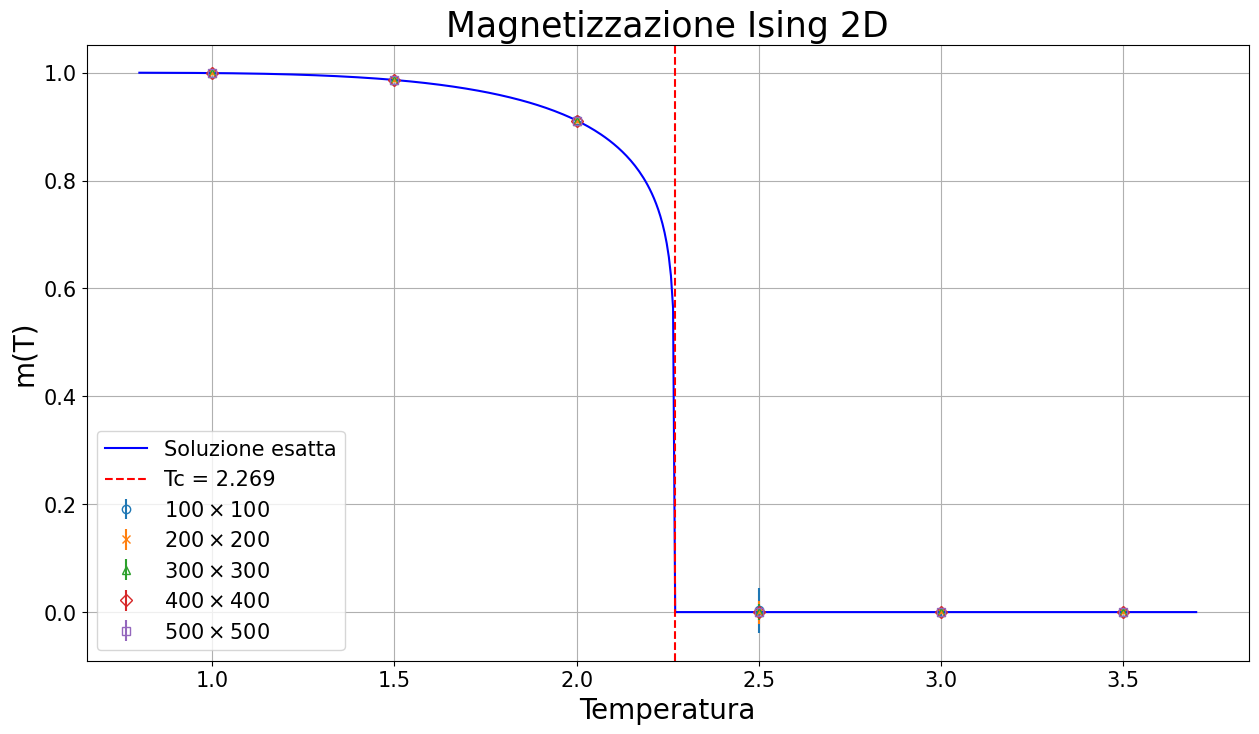
\includegraphics[width=\textwidth]{Immagini/simIsing2D/magn.png}
    \caption{Magnetizzazione modello di Ising 2D: h = 0.0.}
    \label{fig: magn_Ising2D}
\end{figure}

Dato che la maggior parte degli spin sono allineati a bassa temperatura, l'energia interna assume in quella regione il suo valor minimo. 
E' possibile apprezzare $U/N$ tenda a -2, poichè i 4 "legami" che ogni spin presenta con i propri primi vicini sono condivisi con altri 
momenti magnetici. Nel momento in cui $J\,=\,1.0$, l'energia del singolo legame è unitaria e va divisa a metà sui due spin coinvolti nel 
legame.

\begin{figure}[H]
    \centering
    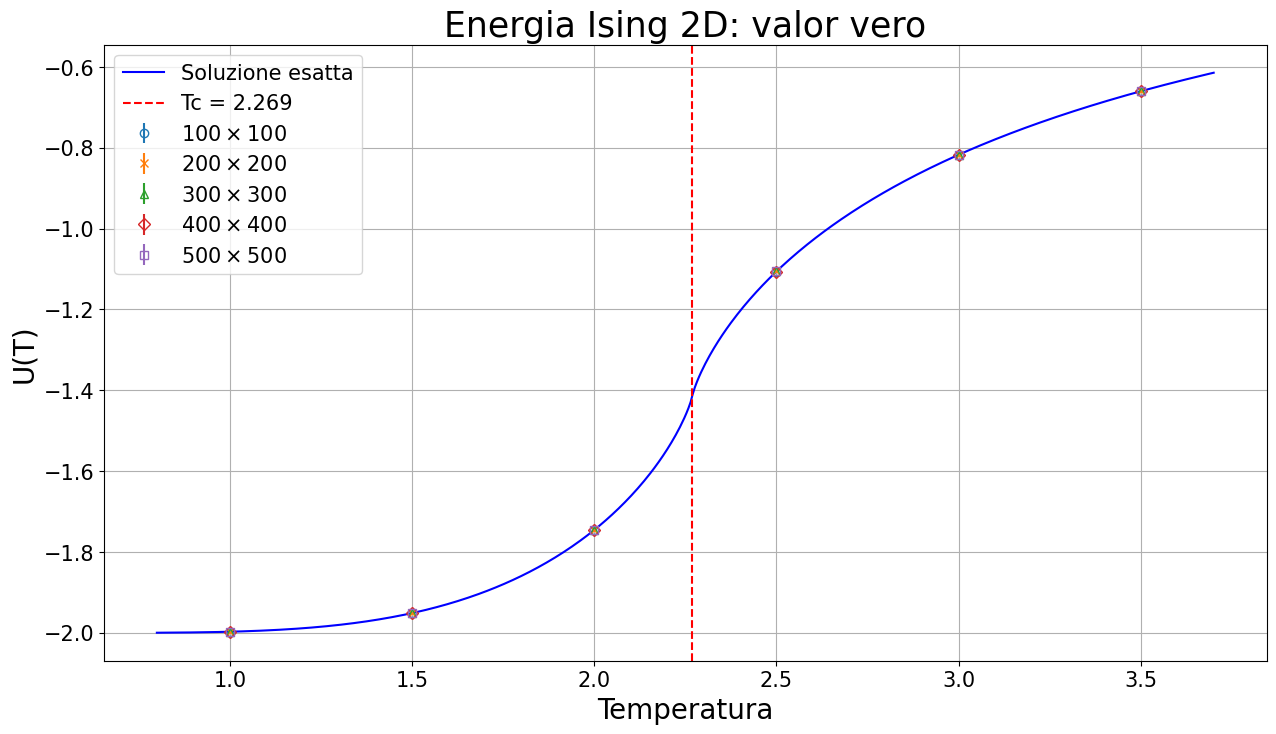
\includegraphics[width=\textwidth]{Immagini/simIsing2D/ene.png}
    \caption{Energia modello di Ising 2D: h = 0.0.}
    \label{fig: ene_Ising2D}
\end{figure}



\subsection{Studio del punto critico}
